\documentclass[12pt,a4paper]{article}

% --- PAKET DASAR ---
\usepackage[utf8]{inputenc}
\usepackage[T1]{fontenc}
\usepackage[bahasa]{babel}
\usepackage{lmodern}

% --- GEOMETRI & TATA LETAK ---
\usepackage[a4paper, landscape, margin=2cm, headheight=10pt]{geometry}

% --- TABEL ---
\usepackage{longtable}
\usepackage{booktabs}
\usepackage{array}
\usepackage{ragged2e}

% --- LAIN-LAIN ---
\usepackage{enumitem}
\usepackage{amsmath}
\usepackage{fancyhdr}
\usepackage{hyperref}
\usepackage{graphicx}
\usepackage{float}
\usepackage{amsfonts}
\usepackage{amssymb}
\usepackage{setspace}
\usepackage{titlesec}
\titleformat{\section}
  {\normalfont\centering\bfseries\Large}
  {}{0pt}{}

\titleformat{\subsection}
  {\normalfont\centering\bfseries\normalsize}
  {}{0pt}{}

\titleformat{\subsubsection}
  {\normalfont\raggedright\bfseries\normalsize}
  {}{0pt}{}
  [\vspace{-0.5em}]

% --- PENGATURAN PARAGRAF ---
\usepackage{ragged2e} % untuk \justifying
\usepackage{indentfirst} % paragraf pertama ikut inden
\setlength{\parindent}{1.25cm} % panjang inden
\setlength{\parskip}{0.75em}   % jarak antar paragraf
\renewcommand{\baselinestretch}{1.5} % spasi antar baris 1.5x
\justifying

% --- PENGATURAN KUSTOM ---
\newcolumntype{P}[1]{>{\RaggedRight\arraybackslash}p{#1}}
\setlist[itemize]{nosep, leftmargin=*}
\setlist[enumerate]{nosep, leftmargin=*}
\newlength{\colwidth}
\setlength{\colwidth}{0.31\textwidth}

% --- HEADER / FOOTER ---
\pagestyle{fancy}
\fancyhf{}
\fancyhead[L]{Research Model Canvas}
\fancyhead[R]{Pangeran Juhrifar Jafar / H071231056}
\fancyfoot[C]{\thepage}
\renewcommand{\headrulewidth}{0.4pt}

% ======================================================
\title{
    \section{Sistem Informasi Cerdas Berbasis YOLOv8 untuk Deteksi, Estimasi Ukuran, dan Pelaporan Jalan Berlubang Secara Real-time}
    % Logo Universitas
    \includegraphics[width=5cm]{Logo-Resmi-Unhas-1.png}
}
\author{
    \textbf{Pangeran Juhrifar Jafar} \\
    NIM: H071231056 \\
    Program Studi Sistem Informasi \\
    Fakultas Matematika dan Ilmu Pengetahuan Alam \\
    Universitas Hasanuddin
}
\date{}


% ======================================================
\begin{document}
\maketitle
\small
\centering
\setlength{\LTpre}{0pt}
\setlength{\LTpost}{0pt}

% ======================================================
% === TABEL 1: State of the Art - Masalah - Kontribusi ===
% ======================================================
\begin{longtable}{@{} P{\colwidth} P{\colwidth} P{\colwidth} @{}}

\multicolumn{3}{c}{\centering\Large\bfseries Research Model Canvas} \\[0.5em]

\caption{Tinjauan Pustaka, Masalah Penelitian, dan Kontribusi} \\
\toprule
\textbf{Tinjauan Pustaka / State of the Art} &
\textbf{Masalah Penelitian} &
\textbf{Kontribusi / Kebaruan} \\
\midrule
\endfirsthead
\toprule
\textbf{Tinjauan Pustaka / State of the Art} &
\textbf{Masalah Penelitian} &
\textbf{Kontribusi / Kebaruan} \\
\midrule
\endhead
\bottomrule
\endfoot

\begin{itemize}
    \item \textbf{Deteksi Objek:} YOLOv8 (Gorro et al., 2024) terbukti akurat untuk deteksi \textit{pothole}.
    \item \textbf{Estimasi Kedalaman:} Wang et al. (2025) mengintegrasikan DepthAnything V2 dan \textit{temporal filtering} (Kalman Filter).
    \item \textbf{Tantangan:} \textit{Scale ambiguity} pada estimasi monokular (Ranftl et al., 2021).
    \item \textbf{Tracking:} BoT-SORT digunakan untuk pelacakan objek yang \textit{robust} (Aharon et al., 2022).
    \item \textbf{GAP:} Belum ada sistem \textit{end-to-end} yang menggabungkan deteksi (YOLOv8) + estimasi ukuran (DepthAnything V2) + \textit{scale recovery} + pelaporan API secara simultan.
\end{itemize} &

\begin{itemize}
    \item \textbf{Keterbatasan Metode Konvensional:} Inspeksi manual lambat, subjektif, tidak efisien, dan reaktif.
    \item \textbf{Fragmentasi Sistem:} Belum ada sistem terintegrasi yang menggabungkan deteksi, pengukuran, dan pelaporan otomatis secara \textit{real-time}.
    \item \textbf{Tantangan Teknis:} Sulit mengukur dimensi (diameter dan kedalaman) secara akurat dari citra kamera monokular.
    \item \textbf{Kebutuhan Mendesak:} Diperlukan sistem \textit{real-time} dengan latensi rendah.
\end{itemize} &

\begin{itemize}
    \item \textbf{Integrasi Terpadu:} Sistem \textit{end-to-end} pertama yang menggabungkan YOLOv8, DepthAnything V2, \textit{scale recovery}, dan API pelaporan.
    \item \textbf{Estimasi Ukuran yang Robust:} Menggunakan \textit{robust statistics} (median, percentile, IQR).
    \item \textbf{Pengukuran Stabil:} \textit{Kalman Filter} menstabilkan hasil diameter dan kedalaman dari waktu ke waktu.
\end{itemize}

\end{longtable}

\vspace{1cm}

% ======================================================
% === TABEL 2: Rumusan, Tujuan, Hasil ===
% ======================================================
\begin{longtable}{@{} P{\colwidth} P{\colwidth} P{\colwidth} @{}}
\caption{Rumusan Masalah, Tujuan, dan Hasil Penelitian} \\
\toprule
\textbf{Rumusan Masalah} &
\textbf{Tujuan Penelitian} &
\textbf{Hasil / Artefak Penelitian} \\
\midrule
\endfirsthead
\toprule
\textbf{Rumusan Masalah} &
\textbf{Tujuan Penelitian} &
\textbf{Hasil / Artefak Penelitian} \\
\midrule
\endhead
\bottomrule
\endfoot

\begin{enumerate}
    \item Bagaimana merancang model YOLOv8 untuk mendeteksi jalan berlubang secara akurat dan \textit{real-time}?
    \item Bagaimana mengestimasi diameter (2D) dan kedalaman (3D) dari citra monokular?
    \item Bagaimana merancang sistem REST API untuk pelaporan otomatis ke \textit{dashboard}?
\end{enumerate} &

\begin{itemize}
    \item Mengimplementasikan YOLOv8n untuk deteksi \textit{real-time}.
    \item Mengembangkan metode estimasi ukuran menggunakan DepthAnything V2 + \textit{scale recovery}.
    \item Mengimplementasikan BoT-SORT dan Kalman Filter untuk stabilitas pengukuran.
    \item Menggunakan \textit{robust statistics} untuk mengurangi \textit{noise}.
    \item Merancang REST API untuk pelaporan otomatis.
\end{itemize} &

\begin{itemize}
    \item Model YOLOv8 terlatih (.pt) untuk deteksi \textit{pothole}.
    \item Sistem estimasi ukuran terintegrasi.
    \item Aplikasi REST API berbasis FastAPI.
    \item Dashboard monitoring \textit{real-time}.
    \item Dokumentasi teknis dan laporan penelitian.
\end{itemize}

\end{longtable}

\vspace{1cm}

% ======================================================
% === TABEL 3: Judul, Metodologi, Evaluasi ===
% ======================================================
\begin{longtable}{@{} P{\colwidth} P{\colwidth} P{\colwidth} @{}}
\caption{Judul, Metodologi, dan Metode Evaluasi Penelitian} \\
\toprule
\textbf{Judul Penelitian} &
\textbf{Metodologi Penelitian} &
\textbf{Metode Evaluasi / Validasi} \\
\midrule
\endfirsthead
\toprule
\textbf{Judul Penelitian} &
\textbf{Metodologi Penelitian} &
\textbf{Metode Evaluasi / Validasi} \\
\midrule
\endhead
\bottomrule
\endfoot

\textbf{Sistem Informasi Cerdas untuk Deteksi, Estimasi Ukuran, dan Pelaporan Otomatis Jalan Berlubang Secara Real-time Menggunakan YOLOv8} &

\begin{itemize}
    \item \textbf{Metode:} Design Science Research (DSR).
    \item \textbf{Pendekatan:} Rancang Bangun, Eksperimental, dan Kuantitatif.
    \item \textbf{Pipeline:} Input Frame $\rightarrow$ Undistort $\rightarrow$ YOLOv8 (Deteksi) $\rightarrow$ DepthAnything V2 dan Depth Mapping(Depth Relatif) $\rightarrow$ Scale Recovery $\rightarrow$ Perhitungan Ukuran $\rightarrow$ BoT-SORT $\rightarrow$ Kalman Filter $\rightarrow$ Output JSON (via API).
\end{itemize} &

\begin{itemize}
    \item \textbf{Evaluasi Kuantitatif:}
    \begin{itemize}
        \item \textbf{Metrik Deteksi:} mAP, Precision, Recall.
        \item \textbf{Metrik Estimasi:} MAE dan RMSE.
        \item \textbf{Metrik Performa:} FPS dan \textit{Latency}.
    \end{itemize}
    \item \textbf{Analisis Eksperimental:}
    \begin{itemize}
        \item \textit{Ablation Study} untuk tiap komponen.
        \item Perbandingan dengan \textit{state-of-the-art}.
        \item Validasi dunia nyata (\textit{ground truth} manual).
    \end{itemize}
\end{itemize}

\end{longtable}

% ======================================================
% BAB 1 PENDAHULUAN
% ======================================================

\clearpage
\raggedright % Reset alignment ke kiri
\fancyhead[L]{BAB I PENDAHULUAN}
\fancyhead[R]{Pangeran Juhrifar Jafar / H071231056}

\onehalfspacing

\section*{BAB I PENDAHULUAN}
\addcontentsline{toc}{section}{BAB I PENDAHULUAN}

\subsection*{1.1 Latar Belakang}
Infrastruktur jalan merupakan fondasi fundamental bagi pembangunan ekonomi dan sosial suatu negara. Jalan yang berkualitas baik tidak hanya memfasilitasi mobilitas masyarakat, tetapi juga mendukung pertumbuhan ekonomi, aksesibilitas layanan publik, dan konektivitas antarwilayah. Dalam konteks pembangunan berkelanjutan, infrastruktur jalan yang memadai menjadi indikator penting kemajuan suatu bangsa dan kesejahteraan masyarakatnya.

Indonesia sebagai negara kepulauan dengan geografi yang kompleks menghadapi tantangan besar dalam pemeliharaan infrastruktur jalan. Data Kementerian Pekerjaan Umum dan Perumahan Rakyat menunjukkan bahwa dari total 496.000 km jalan di Indonesia, sekitar 30\% berada dalam kondisi rusak ringan hingga berat. Masalah jalan berlubang (\textit{potholes}) menjadi fenomena yang sangat umum, terutama di daerah dengan curah hujan tinggi dan beban lalu lintas yang berat. Kondisi ini tidak hanya mengganggu kenyamanan berkendara, tetapi juga menimbulkan risiko keselamatan yang serius dan kerugian ekonomi yang signifikan.

Perkembangan teknologi informasi dan komunikasi telah membuka peluang baru dalam mengatasi permasalahan infrastruktur jalan. Teknologi \textit{Computer Vision} dan \textit{Artificial Intelligence} (AI) menawarkan solusi inovatif untuk deteksi otomatis kerusakan jalan secara real-time. Kemajuan dalam bidang \textit{Deep Learning}, khususnya \textit{Convolutional Neural Networks} (CNN), telah merevolusi kemampuan sistem untuk mengenali dan menganalisis kondisi jalan secara akurat dan efisien.

Beberapa negara maju telah mengimplementasikan sistem deteksi kerusakan jalan berbasis AI dengan hasil yang menggembirakan. Singapura menggunakan sistem \textit{Smart Nation} yang mengintegrasikan sensor dan kamera untuk monitoring infrastruktur secara real-time. Jepang mengembangkan sistem \textit{Road Damage Detection} menggunakan \textit{Machine Learning} untuk mengidentifikasi berbagai jenis kerusakan jalan. Di Indonesia, beberapa kota besar seperti Jakarta dan Surabaya telah mulai mengadopsi teknologi \textit{smart city}, namun implementasi sistem deteksi kerusakan jalan yang komprehensif masih terbatas dan belum terintegrasi dengan baik.

Metode konvensional deteksi kerusakan jalan di Indonesia masih mengandalkan laporan manual dari masyarakat dan inspeksi lapangan oleh petugas, yang memiliki keterbatasan dalam hal kecepatan, akurasi, dan cakupan. Proses ini bersifat reaktif, subjektif, dan seringkali tidak tepat waktu. Terdapat gap yang signifikan antara kebutuhan pemeliharaan jalan yang proaktif dengan kemampuan deteksi yang tersedia. Peluang besar terbuka untuk mengembangkan sistem otomatis yang dapat mendeteksi, mengukur, dan melaporkan kerusakan jalan secara real-time dengan akurasi tinggi.

Sistem informasi memainkan peran krusial dalam mengintegrasikan teknologi deteksi kerusakan jalan dengan proses pengambilan keputusan yang efektif. Melalui \textit{Application Programming Interface} (API) dan \textit{dashboard} interaktif, data hasil deteksi dapat diolah, dianalisis, dan disajikan kepada stakeholder dalam format yang mudah dipahami. Sistem informasi yang terintegrasi memungkinkan otomasi proses pelaporan, prioritisasi perbaikan, dan monitoring progress secara real-time, sehingga mentransformasi manajemen infrastruktur jalan dari pendekatan reaktif menjadi proaktif.

Penelitian sebelumnya telah menunjukkan potensi besar teknologi \textit{Deep Learning} dalam deteksi kerusakan jalan. Gorro et al. (2024) berhasil mengimplementasikan YOLOv8 dengan augmentasi data untuk deteksi lubang jalan dengan akurasi tinggi. Wang et al. (2025) mengembangkan sistem terintegrasi yang menggabungkan estimasi kedalaman monokular dengan \textit{temporal filtering} untuk pengukuran ukuran kerusakan yang akurat. Hoseini et al. (2024) mendemonstrasikan efektivitas arsitektur \textit{deep learning} untuk deteksi objek real-time pada kendaraan otonom. Penelitian-penelitian ini memberikan fondasi teoretis yang kuat untuk pengembangan sistem yang lebih komprehensif.

Berdasarkan analisis gap dan peluang yang ada, penelitian ini bertujuan untuk mengembangkan sistem informasi cerdas yang mengintegrasikan teknologi YOLOv8 untuk deteksi jalan berlubang secara real-time, estimasi ukuran kerusakan menggunakan \textit{depth estimation} monokular, dan sistem pelaporan otomatis melalui REST API. Sistem ini diharapkan dapat mengatasi keterbatasan metode konvensional dengan menyediakan solusi yang akurat, efisien, dan dapat diimplementasikan secara praktis untuk mendukung program \textit{smart city} dan pembangunan infrastruktur berkelanjutan di Indonesia.

\subsection*{1.2 Identifikasi Masalah}
Berdasarkan analisis latar belakang yang telah diuraikan, dapat diidentifikasi beberapa permasalahan mendasar yang menjadi fokus penelitian ini:

\textbf{Permasalahan Utama:}
\begin{enumerate}
    \item \textbf{Keterbatasan Metode Konvensional:} Sistem deteksi kerusakan jalan yang ada saat ini masih mengandalkan laporan manual dan inspeksi lapangan, yang memiliki keterbatasan dalam hal kecepatan, akurasi, dan cakupan geografis.
    \item \textbf{Tantangan Teknis Depth Estimation:} Pengukuran dimensi kerusakan jalan (diameter dan kedalaman) dari citra monokular menghadapi tantangan skala absolut, di mana model deep learning umumnya hanya menghasilkan estimasi kedalaman relatif.
    \item \textbf{Integrasi Sistem yang Terfragmentasi:} Belum ada sistem terintegrasi yang dapat menggabungkan deteksi, pengukuran, dan pelaporan kerusakan jalan dalam satu platform yang efisien dan dapat diakses oleh berbagai stakeholder.
    \item \textbf{Kebutuhan Real-time Processing:} Aplikasi praktis memerlukan sistem yang dapat beroperasi secara real-time dengan latensi rendah, terutama untuk implementasi pada kendaraan yang bergerak.
    \item \textbf{Gap Implementasi di Indonesia:} Meskipun teknologi sudah tersedia, implementasi sistem deteksi kerusakan jalan berbasis AI di Indonesia masih terbatas dan belum terintegrasi dengan sistem manajemen infrastruktur yang ada.
\end{enumerate}

\subsection*{1.3 Rumusan Masalah}
Berdasarkan identifikasi masalah yang telah diuraikan, rumusan masalah dalam penelitian ini adalah:
\begin{enumerate}
    \item Bagaimana merancang dan mengimplementasikan model \textbf{YOLOv8} untuk dapat mendeteksi jalan berlubang secara akurat dan \textit{real-time} dari input video kamera dalam berbagai kondisi jalan?
    \item Bagaimana mengembangkan metode untuk mengestimasi \textbf{diameter (2D)} dan \textbf{kedalaman (3D)} lubang secara akurat dan simultan dari citra kamera monokular dengan mengatasi tantangan skala absolut pada depth estimation?
    \item Bagaimana merancang arsitektur sistem yang dapat mengirimkan data hasil deteksi (koordinat GPS, ukuran, \textit{timestamp}) secara otomatis melalui \textbf{REST API} ke sebuah \textit{dashboard} pemantauan?
\end{enumerate}

\subsection*{1.4 Tujuan Penelitian}
Tujuan dari penelitian ini adalah:
\begin{enumerate}
    \item Mengimplementasikan sistem deteksi jalan berlubang secara \textit{real-time} menggunakan model YOLOv8 (varian ringan seperti YOLOv8n atau YOLOv8s untuk latensi rendah).
    \item Mengembangkan metode terintegrasi untuk mengestimasi \textbf{diameter} dan \textbf{kedalaman} lubang secara simultan menggunakan estimasi kedalaman monokular berbasis deep learning (DepthAnything V2) dengan penerapan \textbf{scale recovery} untuk akurasi metrik absolut.
    \item Mengimplementasikan sistem pelacakan objek (BoT-SORT) dan pemfilteran temporal (Kalman Filter) untuk meningkatkan stabilitas dan akurasi pengukuran.
    \item Menerapkan teknik \textbf{robust statistics} (median, percentile, outlier removal) untuk mengatasi noise pada depth map.
    \item Merancang dan membuat prototipe \textbf{REST API} untuk mengirimkan data hasil deteksi ke sebuah \textit{dashboard} simulasi pihak berwenang.
\end{enumerate}

\subsection*{1.5 Manfaat Penelitian}
Penelitian ini diharapkan memberikan manfaat:
\begin{enumerate}
    \item \textbf{Bagi Pemerintah/Otoritas Jalan:} Menyediakan alat bantu pengambilan keputusan yang berbasis data \textit{real-time} untuk pemeliharaan jalan yang lebih efisien, proaktif, dan terukur dengan klasifikasi severity otomatis.
    \item \textbf{Bagi Masyarakat:} Meningkatkan keselamatan dan kenyamanan berkendara dengan mempercepat proses identifikasi dan perbaikan jalan yang rusak.
    \item \textbf{Bagi Akademisi:} Memberikan kontribusi berupa prototipe sistem \textit{end-to-end} dengan analisis mendalam tentang tantangan implementasi depth estimation monokular, solusi scale recovery, dan best practices untuk aplikasi real-world.
\end{enumerate}

\subsection*{1.6 Signifikansi Penelitian}
Penelitian ini memiliki signifikansi yang tinggi dalam beberapa aspek:

\textbf{Signifikansi Teoritis:}
\begin{itemize}
    \item Memberikan kontribusi dalam pengembangan metodologi depth estimation monokular untuk aplikasi infrastruktur jalan
    \item Mengembangkan framework terintegrasi yang menggabungkan computer vision, deep learning, dan sistem informasi
    \item Menyediakan solusi untuk tantangan scale recovery dalam depth estimation monokular
\end{itemize}

\textbf{Signifikansi Praktis:}
\begin{itemize}
    \item Menyediakan solusi teknologi yang dapat diimplementasikan secara langsung oleh otoritas jalan
    \item Mengurangi biaya operasional dan meningkatkan efisiensi pemeliharaan infrastruktur
    \item Meningkatkan kualitas layanan publik melalui sistem monitoring yang lebih baik
\end{itemize}

\textbf{Signifikansi Sosial:}
\begin{itemize}
    \item Meningkatkan keselamatan berkendara dan mengurangi risiko kecelakaan
    \item Meningkatkan kualitas hidup masyarakat melalui infrastruktur jalan yang lebih baik
    \item Mendukung program smart city dan pembangunan berkelanjutan
\end{itemize}

\textbf{Signifikansi Ekonomi:}
\begin{itemize}
    \item Mengurangi biaya perawatan kendaraan akibat kerusakan jalan
    \item Meningkatkan efisiensi logistik dan transportasi
    \item Menciptakan peluang bisnis baru dalam bidang teknologi infrastruktur
\end{itemize}

\subsection*{1.7 Batasan Masalah}
Penelitian ini dibatasi pada:
\begin{enumerate}
    \item \textbf{Model yang Digunakan:} Hanya menggunakan YOLOv8n (nano version) untuk deteksi objek
    \item \textbf{Jenis Kerusakan:} Fokus pada deteksi lubang jalan (potholes) saja, tidak termasuk jenis kerusakan jalan lainnya
    \item \textbf{Kondisi Lingkungan:} Evaluasi dilakukan pada kondisi normal (siang hari, cuaca cerah)
    \item \textbf{Platform Implementasi:} Sistem diimplementasikan pada platform desktop/laptop
    \item \textbf{Area Geografis:} Testing dilakukan di area terbatas dengan karakteristik jalan yang spesifik
    \item \textbf{Kamera:} Menggunakan kamera monokular standar, bukan kamera stereo atau multi-view
    \item \textbf{Dataset:} Menggunakan dataset yang tersedia secara publik dengan anotasi terbatas
\end{enumerate}


% ======================================================
% BAB II HASIL PELATIHAN MODEL
% ======================================================

\clearpage
\raggedright
\fancyhead[L]{BAB II HASIL PELATIHAN MODEL}
\fancyhead[R]{Pangeran Juhrifar Jafar / H071231056}

\onehalfspacing

\section*{BAB II HASIL PELATIHAN MODEL}
\addcontentsline{toc}{section}{BAB II HASIL PELATIHAN MODEL}

\subsection*{2.1 Konfigurasi Pelatihan}

Pelatihan model YOLOv8n untuk deteksi jalan berlubang dilakukan melalui dua tahap utama: pelatihan awal (\textit{initial training}) dan \textit{fine-tuning}. Model yang digunakan adalah YOLOv8n (nano version) yang dipilih karena efisiensi komputasinya yang tinggi, sehingga cocok untuk aplikasi \textit{real-time}.

\textbf{Konfigurasi Pelatihan Fine-tuning:}
\begin{itemize}
    \item \textbf{Model Base:} YOLOv8n-potholes (best.pt dari pelatihan awal)
    \item \textbf{Epochs:} 50 epoch
    \item \textbf{Batch Size:} 8
    \item \textbf{Image Size:} 640x640 piksel
    \item \textbf{Learning Rate:} 0.01 (dengan decay otomatis)
    \item \textbf{Optimizer:} AdamW (otomatis)
    \item \textbf{Augmentation:} RandAugment, Mosaic, MixUp, Flip
    \item \textbf{Device:} GPU
\end{itemize}

\subsection*{2.2 Dataset}

Dataset yang digunakan untuk pelatihan model diambil dari \textbf{Roboflow Universe}, sebuah platform publik yang menyediakan dataset untuk \textit{object detection}. Dataset yang digunakan adalah \textbf{Pothole Dataset} yang dapat diakses melalui \url{https://public.roboflow.com/object-detection/pothole/1}.

\textbf{Spesifikasi Dataset:}
\begin{itemize}
    \item \textbf{Sumber:} Roboflow Universe - Pothole Dataset
    \item \textbf{Total Images:} 665 gambar
    \item \textbf{Format Anotasi:} YOLO format (YOLOv8) dengan anotasi bounding box
    \item \textbf{Kelas Objek:} Potholes (lubang jalan)
    \item \textbf{Resolusi:} Bervariasi, diresize ke 640x640 piksel untuk pelatihan
    \item \textbf{Data Split:} Dataset dibagi menggunakan proporsi 70/20/10:
    \begin{itemize}
        \item \textbf{Train Set:} 465 gambar (70\%)
        \item \textbf{Validation Set:} 133 gambar (20\%) dengan 330 instance lubang jalan
        \item \textbf{Test Set:} 67 gambar (10\%)
    \end{itemize}
\end{itemize}

Dataset ini telah di-export dalam format YOLOv8 yang kompatibel langsung dengan framework pelatihan YOLOv8. Anotasi bounding box telah dilakukan sebelumnya dan siap digunakan untuk pelatihan model deteksi objek.


\subsection*{2.3 Hasil Evaluasi Model Fine-tuned}

Setelah proses fine-tuning selama 50 epoch, model \textbf{yolov8n-potholes-ft} dievaluasi pada dataset validasi. Hasil evaluasi menunjukkan performa yang baik untuk tahap prototipe sistem deteksi lubang jalan. Berikut adalah metrik evaluasi yang diperoleh:

\begin{table}[h]
\centering
\caption{Hasil Evaluasi Model YOLOv8n-potholes-ft}
\label{tab:hasil-evaluasi}
\begin{tabular}{@{}lcc@{}}
\toprule
\textbf{Metrik} & \textbf{Nilai} & \textbf{Interpretasi} \\
\midrule
\textbf{Precision (P)} & 0.793 & Akurasi tinggi saat model memprediksi lubang \\
\textbf{Recall (R)} & 0.679 & Beberapa lubang kecil masih belum terdeteksi \\
\textbf{mAP@0.5} & 0.775 & Akurasi deteksi bounding box baik \\
\textbf{mAP@0.5-0.95} & 0.502 & Performa pada berbagai threshold IoU \\
\bottomrule
\end{tabular}
\end{table}

\subsection*{2.4 Analisis Hasil Pelatihan}

\subsubsection*{2.4.1 Analisis Metrik Deteksi}

\textbf{Precision (0.793):} Nilai precision yang mencapai 79.3\% menunjukkan bahwa model memiliki akurasi yang tinggi dalam memprediksi lubang jalan. Artinya, ketika model memprediksi suatu objek sebagai lubang jalan, kemungkinan besar prediksi tersebut benar. Tingkat \textit{false positive} yang rendah (sekitar 20.7\%) menunjukkan bahwa model tidak terlalu sering salah mengidentifikasi objek lain sebagai lubang jalan.

\textbf{Recall (0.679):} Nilai recall sebesar 67.9\% menunjukkan bahwa model masih melewatkan beberapa lubang jalan yang sebenarnya ada dalam gambar. Terdapat sekitar 32.1\% lubang jalan yang tidak terdeteksi (\textit{false negative}). Hal ini umum terjadi pada dataset dengan variasi kondisi pencahayaan tinggi dan lubang kecil yang sulit dideteksi.

\textbf{mAP@0.5 (0.775):} Mean Average Precision pada IoU threshold 0.5 sebesar 77.5\% menunjukkan performa yang baik untuk deteksi bounding box. Nilai ini mengindikasikan bahwa model mampu mendeteksi dan melokalisasi lubang jalan dengan akurasi yang memadai.

\textbf{mAP@0.5-0.95 (0.502):} Mean Average Precision pada berbagai threshold IoU (dari 0.5 hingga 0.95) sebesar 50.2\% menunjukkan bahwa model masih memiliki ruang untuk peningkatan, terutama dalam hal akurasi lokalisasi yang lebih ketat. Namun, nilai ini sudah cukup solid untuk tahap prototipe.

\subsubsection*{2.4.2 Analisis Kurva Pelatihan}

Berdasarkan analisis kurva pelatihan (\textit{training curves}):

\begin{itemize}
    \item \textbf{Box Loss, Classification Loss, dan DFL Loss:} Semua loss function menunjukkan penurunan yang stabil sepanjang 50 epoch, mengindikasikan bahwa model terus belajar dengan baik tanpa tanda-tanda \textit{overfitting} yang signifikan.
    
    \item \textbf{Precision \& Recall:} Meskipun mengalami fluktuasi selama pelatihan, tren akhir menunjukkan peningkatan, dengan precision mencapai sekitar 0.79 dan recall sekitar 0.68 pada epoch terakhir.
    
    \item \textbf{mAP@0.5:} Meningkat secara stabil dari sekitar 0.4 pada epoch awal menjadi 0.78 pada epoch akhir, menunjukkan konvergensi yang baik.
    
    \item \textbf{mAP@0.5-0.95:} Meningkat dari nilai awal menjadi sekitar 0.50, menunjukkan peningkatan akurasi pada berbagai tingkat IoU threshold.
\end{itemize}

\begin{figure}[H]
\centering
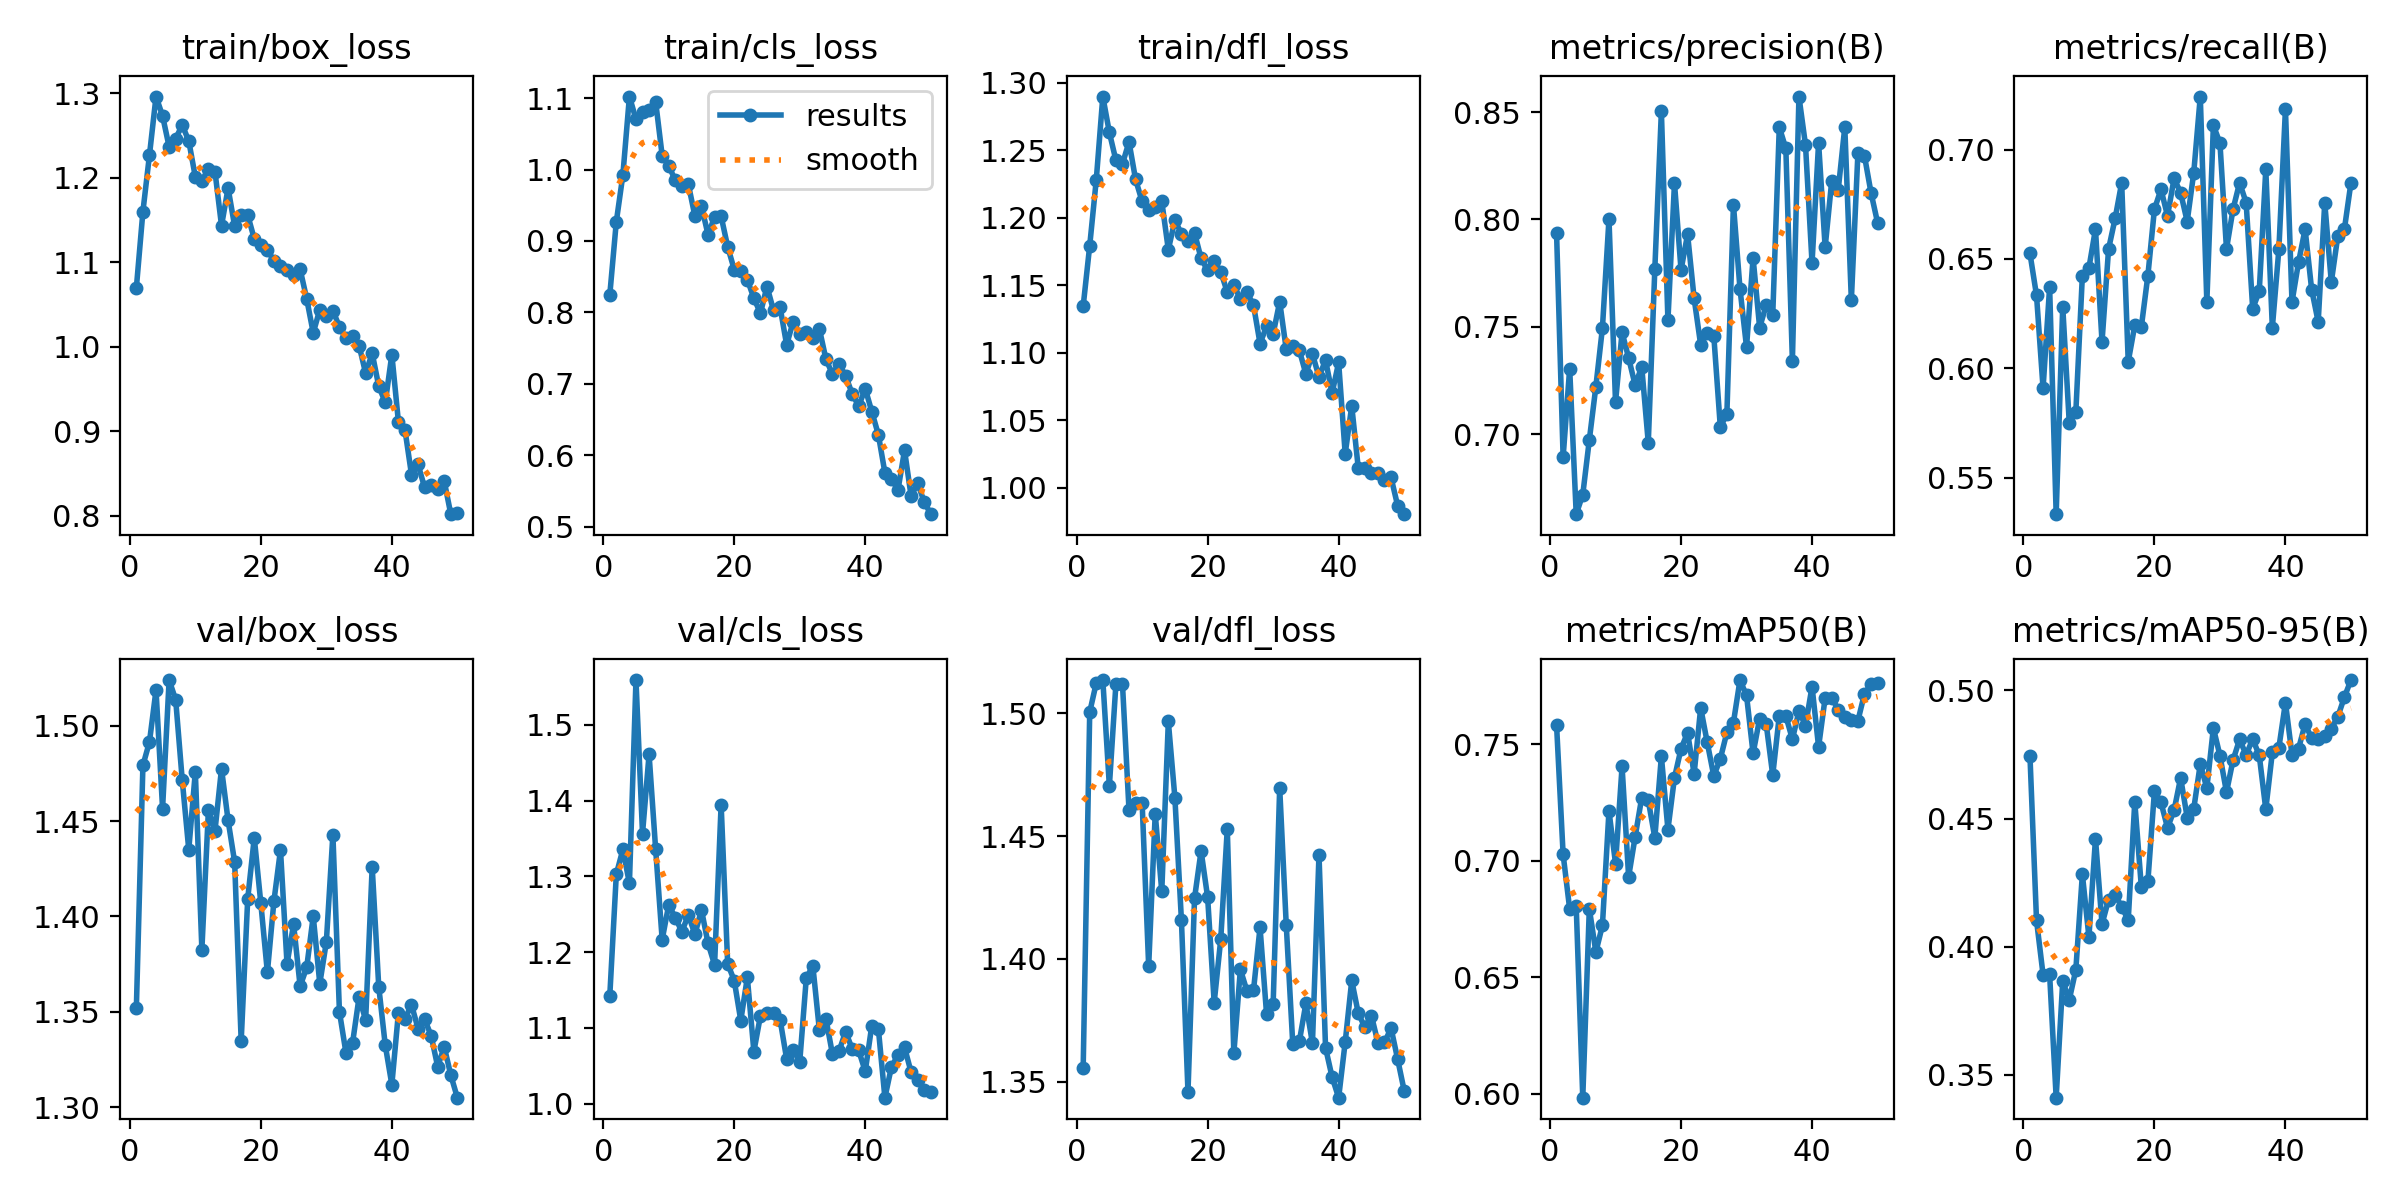
\includegraphics[width=0.9\textwidth]{../runs/detect/yolov8n-potholes-ft/results.png}
\caption{Grafik Hasil Pelatihan Model YOLOv8n-potholes-ft: (a) Box Loss, (b) Classification Loss, (c) DFL Loss, (d) Precision, (e) Recall, (f) mAP@0.5, (g) mAP@0.5-0.95}
\label{fig:training-curves}
\end{figure}

\subsubsection*{2.4.3 Analisis Confusion Matrix}

Dari analisis \textit{confusion matrix}, diperoleh informasi berikut:

\begin{itemize}
    \item \textbf{True Positive (TP):} 246 instance - Prediksi benar sebagai lubang jalan
    \item \textbf{False Negative (FN):} 84 instance - Lubang jalan yang tidak terdeteksi
    \item \textbf{False Positive (FP):} 120 instance - Prediksi salah sebagai lubang jalan
    \item \textbf{Recall (Sensitivitas):} 0.75 (dari confusion matrix normalized)
    \item \textbf{Precision terhadap Background:} 1.00 (sangat tinggi)
\end{itemize}

\begin{figure}[H]
\centering
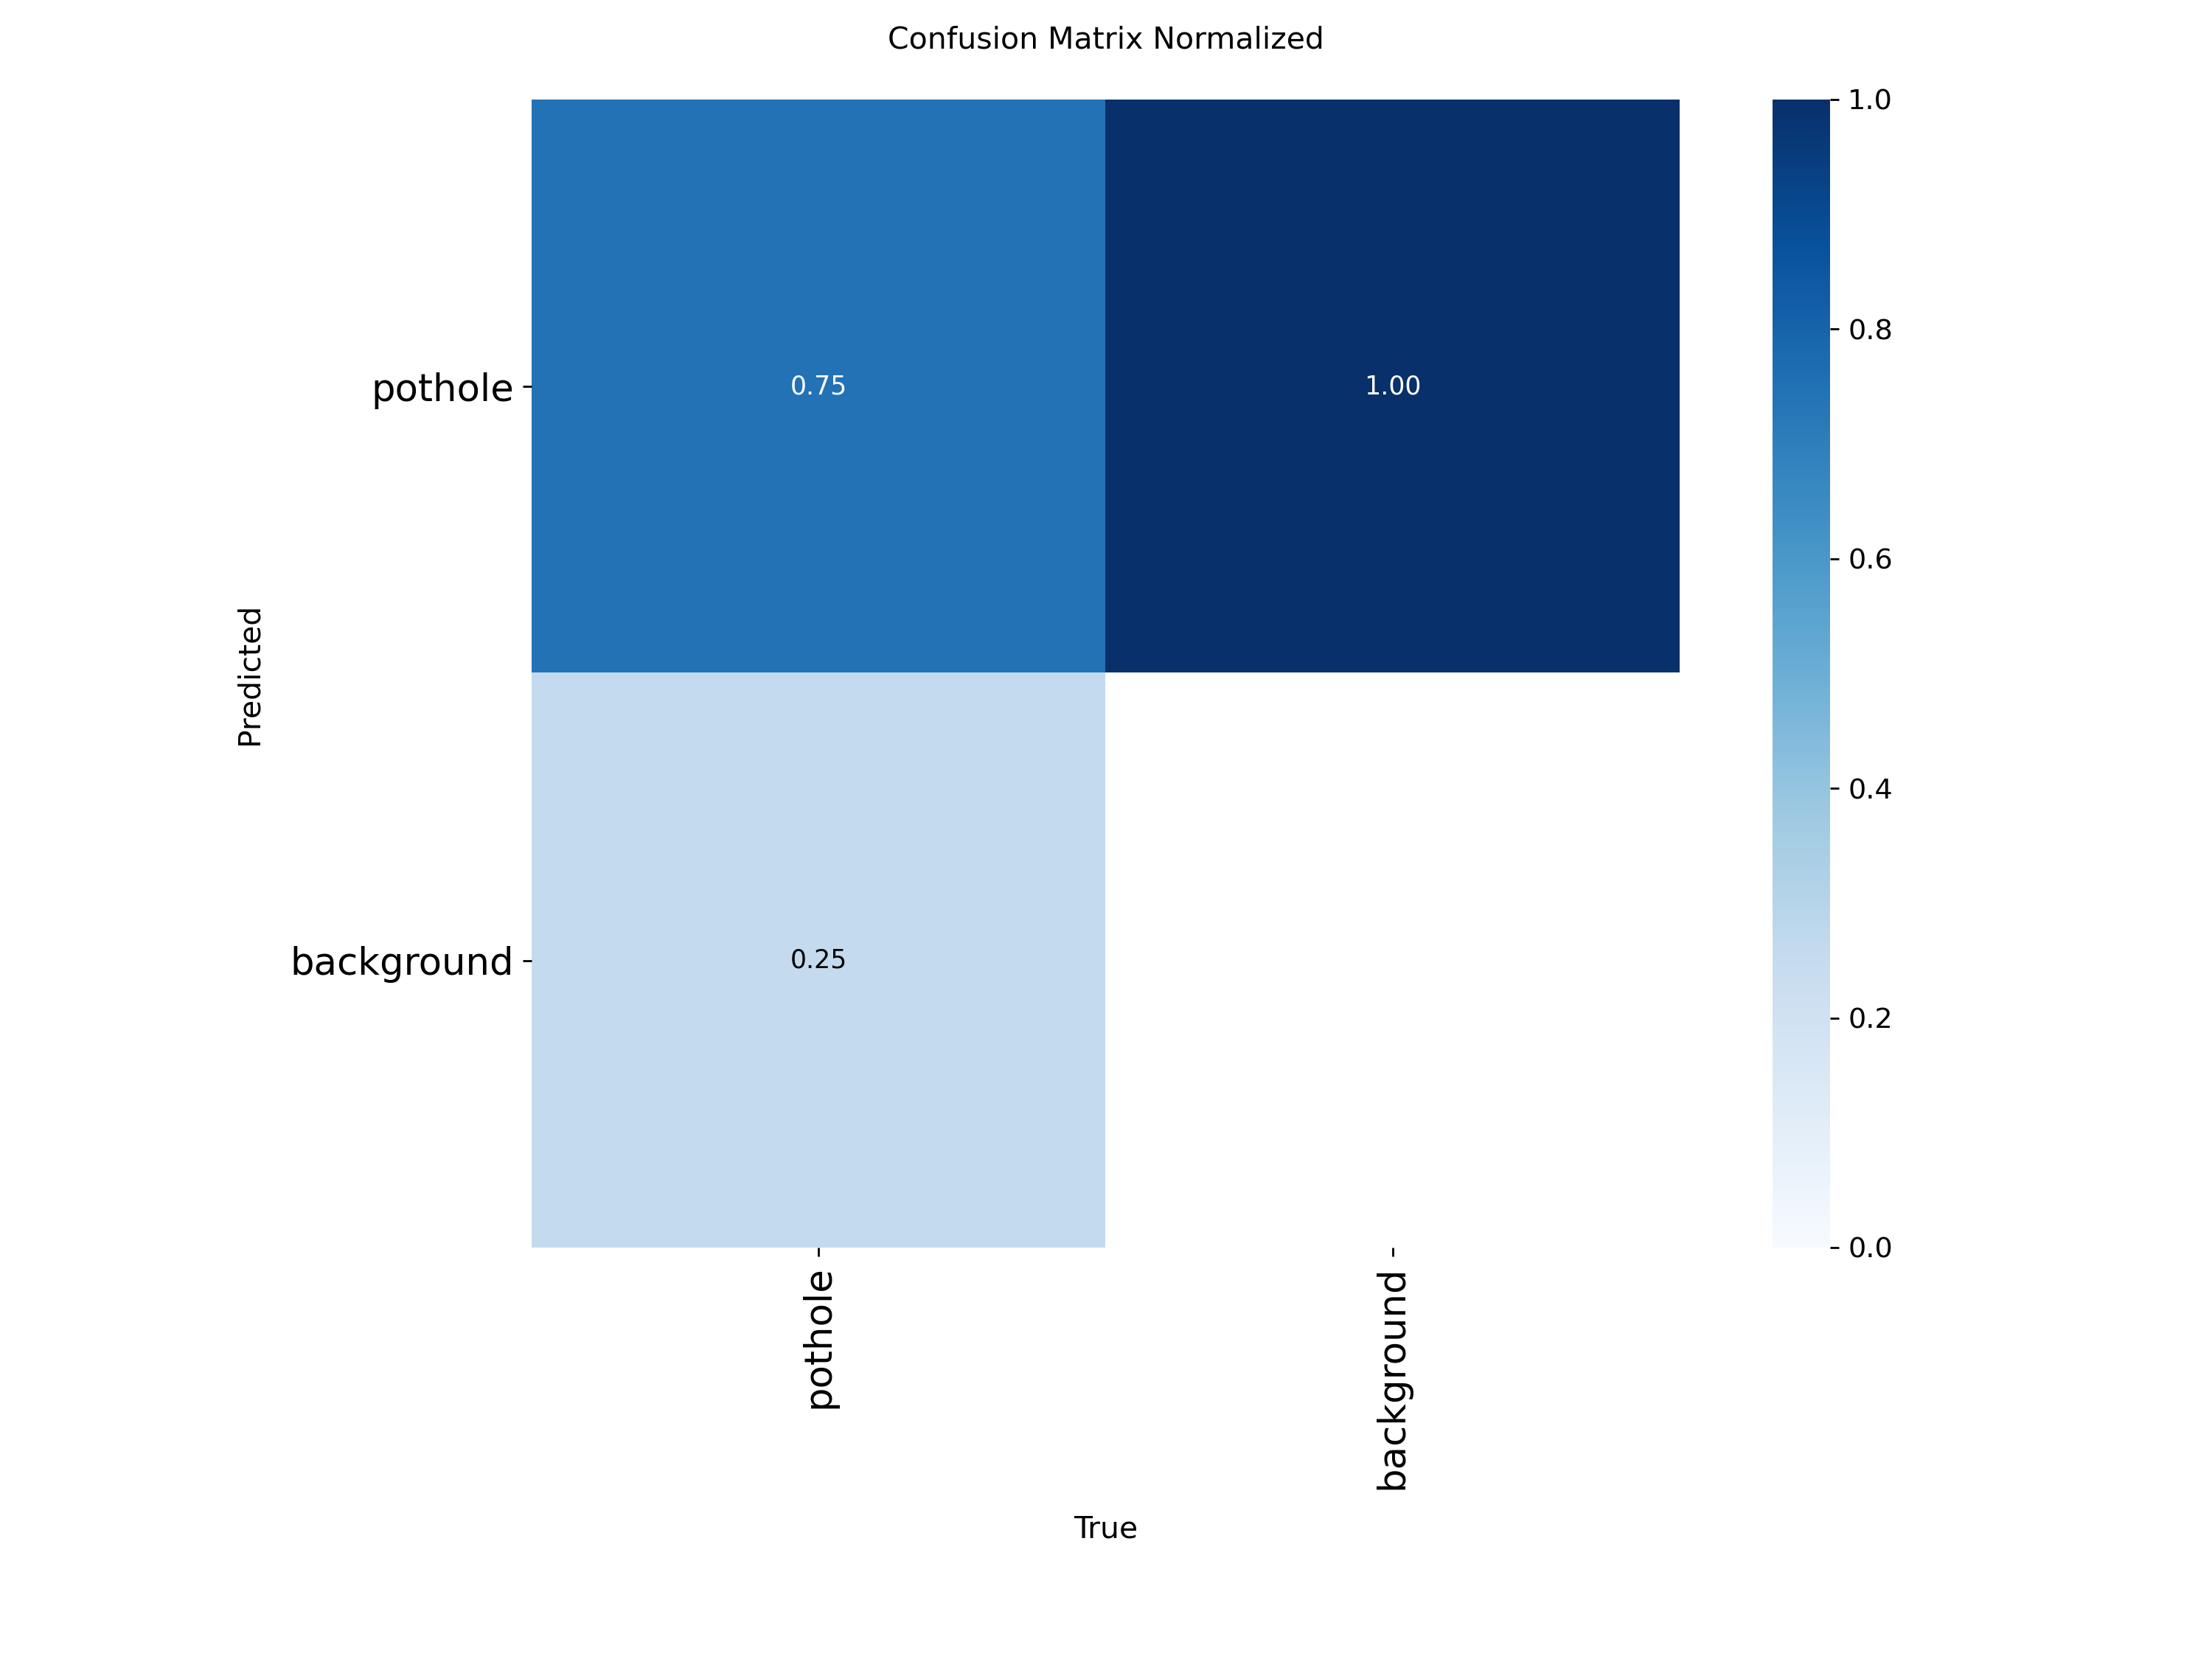
\includegraphics[width=0.6\textwidth]{../runs/detect/yolov8n-potholes-ft/confusion_matrix_normalized.png}
\caption{Confusion Matrix Normalized Model YOLOv8n-potholes-ft}
\label{fig:confusion-matrix}
\end{figure}

\textbf{Interpretasi:} Model menunjukkan karakteristik yang lebih konservatif, yaitu lebih memilih untuk tidak mendeteksi (\textit{miss}) dibandingkan salah mendeteksi (\textit{false positive}). Karakteristik ini umum terjadi pada dataset jalan dengan variasi pencahayaan tinggi dan dapat diterima untuk aplikasi prototipe, karena lebih baik melewatkan beberapa deteksi daripada menghasilkan terlalu banyak alarm palsu.

\subsection*{2.5 Kesimpulan Hasil Pelatihan}

Model hasil fine-tuning \textbf{yolov8n-potholes-ft} menunjukkan peningkatan yang nyata dari model awal dengan keseimbangan yang baik antara precision dan recall. Kinerja model sudah cukup layak untuk tahap prototipe sistem deteksi lubang jalan \textit{real-time}, dengan karakteristik sebagai berikut:

\begin{enumerate}
    \item \textbf{Konvergensi yang Baik:} Model berhasil konvergen tanpa indikasi \textit{overfitting} yang signifikan, ditunjukkan oleh penurunan loss yang stabil pada data training dan validation.
    
    \item \textbf{Akurasi Deteksi Tinggi:} Precision sebesar 79.3\% menunjukkan bahwa model dapat diandalkan dalam memprediksi lubang jalan dengan tingkat kesalahan yang rendah.
    
    \item \textbf{Ruang Peningkatan:} Recall sebesar 67.9\% menunjukkan masih ada peluang untuk meningkatkan kemampuan deteksi, terutama untuk lubang kecil dan dalam kondisi pencahayaan yang sulit.
    
    \item \textbf{Kesiapan untuk Tahap Selanjutnya:} Model sudah siap untuk diintegrasikan dengan komponen sistem lainnya, seperti estimasi kedalaman menggunakan DepthAnything V2 dan sistem pelaporan melalui REST API.
\end{enumerate}

\subsubsection*{2.4.4 Contoh Hasil Prediksi Model}

Berikut adalah contoh hasil prediksi model pada data validasi yang menunjukkan kemampuan model dalam mendeteksi lubang jalan:

\begin{figure}[H]
\centering
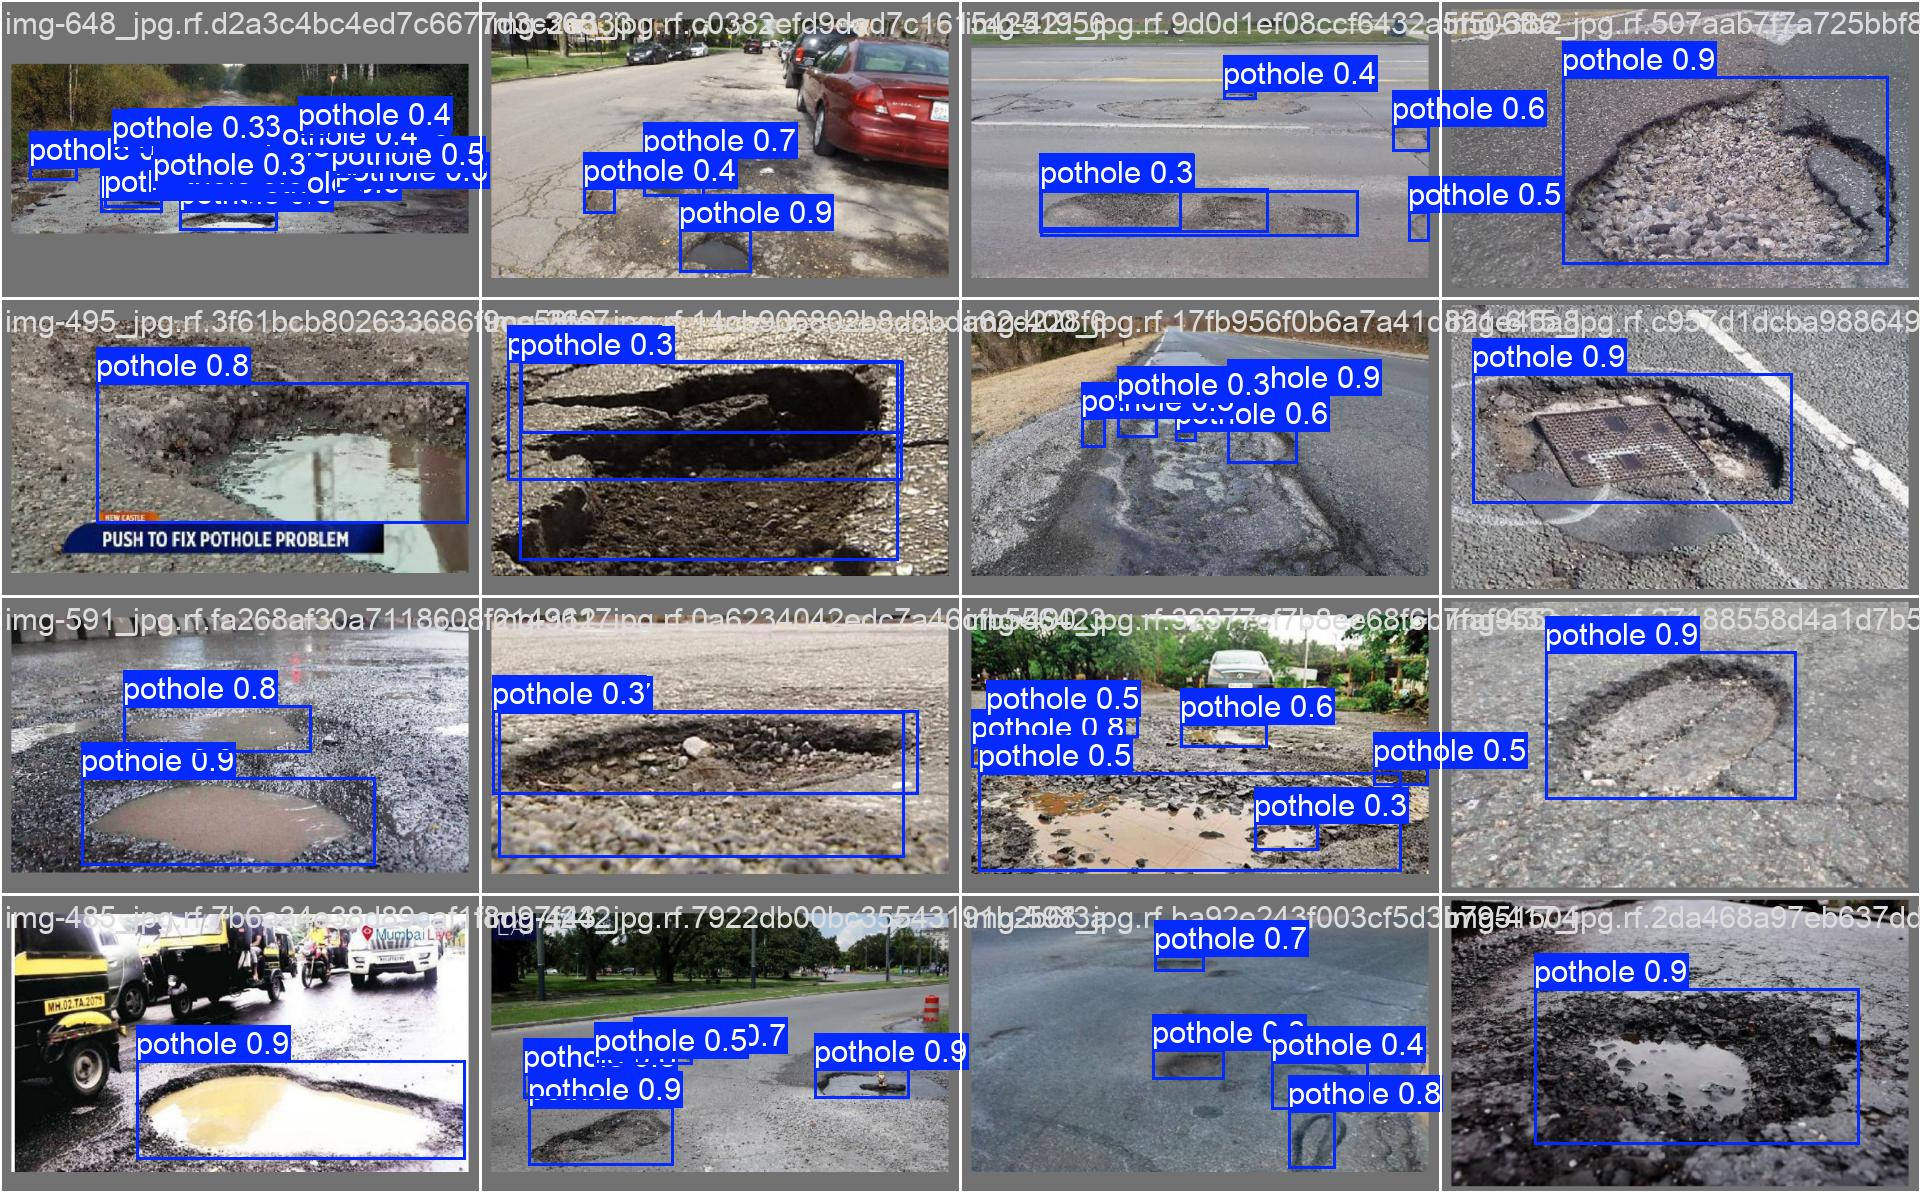
\includegraphics[width=0.8\textwidth]{../runs/detect/yolov8n-potholes-ft/val_batch0_pred.jpg}
\caption{Contoh Hasil Prediksi Model pada Data Validasi}
\label{fig:prediction-example}
\end{figure}

Gambar di atas menunjukkan bahwa model mampu mendeteksi lubang jalan dengan akurat, ditandai dengan bounding box yang mengelilingi area lubang. Model menunjukkan performa yang baik dalam mengidentifikasi berbagai ukuran lubang jalan dengan tingkat confidence yang memadai.

\subsection*{2.5 Kesimpulan Hasil Pelatihan}

Model hasil fine-tuning \textbf{yolov8n-potholes-ft} menunjukkan peningkatan yang nyata dari model awal dengan keseimbangan yang baik antara precision dan recall. Kinerja model sudah cukup layak untuk tahap prototipe sistem deteksi lubang jalan \textit{real-time}, dengan karakteristik sebagai berikut:

\begin{enumerate}
    \item \textbf{Konvergensi yang Baik:} Model berhasil konvergen tanpa indikasi \textit{overfitting} yang signifikan, ditunjukkan oleh penurunan loss yang stabil pada data training dan validation.
    
    \item \textbf{Akurasi Deteksi Tinggi:} Precision sebesar 79.3\% menunjukkan bahwa model dapat diandalkan dalam memprediksi lubang jalan dengan tingkat kesalahan yang rendah.
    
    \item \textbf{Ruang Peningkatan:} Recall sebesar 67.9\% menunjukkan masih ada peluang untuk meningkatkan kemampuan deteksi, terutama untuk lubang kecil dan dalam kondisi pencahayaan yang sulit.
    
    \item \textbf{Kesiapan untuk Tahap Selanjutnya:} Model sudah siap untuk diintegrasikan dengan komponen sistem lainnya, seperti estimasi kedalaman menggunakan DepthAnything V2 dan sistem pelaporan melalui REST API.
\end{enumerate}

\subsection*{2.6 Rekomendasi untuk Peningkatan}

Untuk meningkatkan performa model di masa depan, beberapa rekomendasi yang dapat dilakukan:

\begin{enumerate}
    \item \textbf{Augmentasi Data:} Menerapkan augmentasi yang lebih agresif, terutama untuk variasi pencahayaan (exposure), blur, dan noise untuk meningkatkan robustnes model.
    
    \item \textbf{Tuning Confidence Threshold:} Mengeksplorasi nilai confidence threshold yang lebih rendah (0.2-0.3) untuk meningkatkan recall, dengan mempertimbangkan trade-off terhadap precision.
    
    \item \textbf{Data Collection:} Mengumpulkan lebih banyak data, terutama untuk lubang kecil dan kondisi pencahayaan yang sulit, untuk meningkatkan kemampuan deteksi model.
    
    \item \textbf{Optimasi Model:} Menerapkan optimasi seperti TensorRT untuk deployment pada perangkat edge seperti NVIDIA Jetson, yang dapat meningkatkan kecepatan inferensi tanpa mengorbankan akurasi.
\end{enumerate}

% ======================================================
% DAFTAR PUSTAKA
% ======================================================

\clearpage
\fancyhead[L]{DAFTAR PUSTAKA}
\fancyhead[R]{Pangeran Juhrifar Jafar / H071231056}

\section*{DAFTAR PUSTAKA}
\addcontentsline{toc}{section}{DAFTAR PUSTAKA}

\onehalfspacing

\begin{thebibliography}{99}

\bibitem{albawi2017}
Albawi, S., Mohammed, T. A., \& Al-Zawi, S. (2017). Understanding of a Convolutional Neural Network. \textit{2017 International Conference on Engineering and Technology (ICET)}, 1--6.

\bibitem{lecun2015}
LeCun, Y., Bengio, Y., \& Hinton, G. (2015). Deep Learning. \textit{Nature}, 521(7553), 436--444.

\bibitem{zhao2019}
Zhao, Z. Q., Zheng, P., Xu, S. T., \& Wu, X. (2019). Object Detection with Deep Learning: A Review. \textit{IEEE Transactions on Neural Networks and Learning Systems}, 30(11), 3212--3232.

\bibitem{redmon2016}
Redmon, J., et al. (2016). You Only Look Once: Unified, Real-Time Object Detection. \textit{Proceedings of the IEEE Conference on Computer Vision and Pattern Recognition}, 779--788.

\bibitem{godard2017}
Godard, C., Mac Aodha, O., \& Brostow, G. J. (2017). Unsupervised Monocular Depth Estimation with Left-Right Consistency. \textit{Proceedings of the IEEE Conference on Computer Vision and Pattern Recognition}, 270--279.

\bibitem{laina2016}
Laina, I., et al. (2016). Deeper Depth Prediction with Fully Convolutional Residual Networks. \textit{Proceedings of the IEEE International Conference on 3D Vision}, 239--248.

\bibitem{ranftl2021}
Ranftl, R., Bochkovskiy, A., \& Koltun, V. (2021). Vision Transformers for Dense Prediction. \textit{Proceedings of the IEEE/CVF International Conference on Computer Vision}, 12179--12188.

\bibitem{bewley2016}
Bewley, A., Ge, Z., Ott, L., Ramos, F., \& Upcroft, B. (2016). Simple Online and Realtime Tracking. \textit{2016 IEEE International Conference on Image Processing (ICIP)}, 3464--3468.

\bibitem{aharon2022}
Aharon, N., et al. (2022). BoT-SORT: Robust Associations Multi-Pedestrian Tracking. \textit{arXiv preprint arXiv:2206.14651}.

\bibitem{kalman1960}
Kalman, R. E. (1960). A New Approach to Linear Filtering and Prediction Problems. \textit{Journal of Basic Engineering}, 82(1), 35--45.

\bibitem{fielding2000}
Fielding, R. T. (2000). \textit{Architectural Styles and the Design of Network-based Software Architectures}. Doctoral Dissertation, University of California, Irvine.

\bibitem{richardson2007}
Richardson, L., \& Ruby, S. (2007). \textit{RESTful Web Services}. O'Reilly Media, Inc.

\bibitem{liu1973}
Liu, C. L., \& Layland, J. W. (1973). Scheduling Algorithms for Multiprogramming in a Hard-Real-Time Environment. \textit{Journal of the ACM}, 20(1), 46--61.

\bibitem{kopetz2011}
Kopetz, H. (2011). \textit{Real-Time Systems: Design Principles for Distributed Embedded Applications}. Springer Science \& Business Media.

\bibitem{huber1981}
Huber, P. J. (1981). \textit{Robust Statistics}. John Wiley \& Sons.

\bibitem{shi2016}
Shi, W., Cao, J., Zhang, Q., Li, Y., \& Xu, L. (2016). Edge Computing: Vision and Challenges. \textit{IEEE Internet of Things Journal}, 3(5), 637--646.

\bibitem{satyanarayanan2017}
Satyanarayanan, M. (2017). The Emergence of Edge Computing. \textit{Computer}, 50(1), 30--39.

\bibitem{depthanything2024}
DepthAnything Team. (2024). DepthAnything V2: Dense Prediction Transformer for Monocular Depth Estimation. \textit{arXiv preprint arXiv:2406.09414}.

\end{thebibliography}

\end{document}